\documentclass[11pt]{article}
\usepackage{amsmath}
\usepackage{amssymb}
\usepackage{amsthm}
\usepackage{booktabs}
\usepackage{caption}
\usepackage{enumitem}
\newlist{inlinelist}{enumerate*}{1}
\setlist*[inlinelist]{label=(\arabic*)}
\usepackage[totalwidth=450pt, totalheight=630pt]{geometry}
\usepackage{graphicx}
\PassOptionsToPackage{hyphens}{url} % pass options to url autoloaded by hyperref
\usepackage[pdfencoding=auto, psdextra]{hyperref} % hyperref must be loaded before cleveref
\usepackage{mathrsfs}
\usepackage{multirow}
\usepackage[round]{natbib} % natbib must be loaded before algorithm2e
\usepackage[linesnumbered, ruled]{algorithm2e} % algorithm2e must be loaded before cleveref
\usepackage{cleveref}
\usepackage{subcaption}
\usepackage{tikz}
\usetikzlibrary{calc}
\usepackage{verbatim}
\usepackage{xcolor}

\interfootnotelinepenalty=10000

\captionsetup{width=0.8\textwidth}

\newtheorem{corollary}{Corollary}
\newtheorem{definition}{Definition}
\newtheorem{lemma}[corollary]{Lemma}
\newtheorem{proposition}[corollary]{Proposition}
\newtheorem{theorem}[corollary]{Theorem}

\theoremstyle{definition}
\newtheorem{assumption}{Assumption}
\newtheorem{example}{Example}
\newtheorem*{remark}{Remark}

\newtheoremstyle{custom}{}{}{\itshape}{}{\bfseries}{.}{.5em}{\thmnote{#3}}
\theoremstyle{custom}
\newtheorem*{customthm}{Theorem}

\setlength{\tabcolsep}{1em}
\setlist{listparindent=\parindent, parsep=0pt}

\newcommand{\EE}{\mathbb{E}}
\newcommand{\cF}{\mathcal{F}}
\newcommand{\PP}{\mathbb{P}}
\newcommand{\RR}{\mathbb{R}}
\newcommand{\ZZ}{\mathbb{Z}}
\newcommand{\cH}{\mathcal{H}}
\DeclareMathOperator*{\argmax}{arg\,max}
\DeclareMathOperator*{\se}{se}
\DeclareMathOperator{\sgn}{sign}

\newcommand{\hdelta}{\hat{\delta}}
\newcommand{\hmu}{\hat{\mu}}
\newcommand{\hsigma}{\hat{\sigma}}
\newcommand{\htheta}{\hat{\theta}}
\newcommand{\ao}{\alpha_0}
\newcommand{\gest}{\ge_\text{st}}

\newcommand{\WFcomment}[1]{{\color{red!40!gray} (WF: #1)}}
\newcommand{\KHcomment}[1]{{\color{green!40!gray} (KH: #1)}}

% Uncomment this line to get rid of my comments
% \renewcommand{\WFcomment}[1]{}
% \renewcommand{\KHcomment}[1]{}

\graphicspath{{./fig/}}

\begin{document}

\title{Supplement to ``Statistical Methods for Replicability Assessment''}
\date{\today}
\author{
  Kenneth Hung\thanks{Department of Mathematics, University of California, Berkeley} \and
  William Fithian\thanks{Department of Statistics, University of California, Berkeley}
}
\maketitle

\section{\texorpdfstring{$t$}{t}-tests and ANOVAs}

  Both $t$-tests and $F(1, \cdot)$ ANOVAs, whether they are within-subject or between-subject, one-way or multi-way, can be thought of as testing some contrast $\delta$ of the true cell means. 

  We can construct unbiased estimators $\hdelta$ and $\hsigma^2$ for the contrast and the common variance from the homoscedasticity assumption. The standard error can be written as $\frac{\sigma}{k}$ where $\sigma^2$ is the true variance and $k$ is some known constant determined by the cell sizes. We can now test the null hypothesis $\delta = 0$ using the $t$-statistic $T = k \hdelta / \hsigma$. If there is an effect, i.e.\ $\delta \ne 0$, then $T$ follows the noncentral $t$-distribution
  \[
    T \sim t_{df}\left(k\frac{\delta}{\sigma}\right).
  \]
  We take the effect size $\theta$ to be $\delta / \sigma$.

  For notation, we will use subscripts to indicate the cell. We will use $\mu_i$ (or, $\mu_{ij}$ or $\mu_{ijk}$) to denote the population mean in each cell. For the marginals, we use $*$ to indicated dimensions averaged out. For example, in a $2 \times 3$ ANOVA,
  \[
    \mu_{1*} = \frac{\mu_{11} + \mu_{12} + \mu_{13}}{3}.
  \]
  For designs with between-subject factor(s), the subject can be naturally grouped, we will use $I_i$ (or $I_{ij}$) to indicate these groups. The number of subjects in each is $n_i$ (or $n_{ij}$) respectively. For example, if there are two between-subject factors, each with two levels, we have four groups $I_{11}$, $I_{12}$, $I_{21}$ and $I_{22}$, and their sizes are $n_{11}$, $n_{12}$, $n_{21}$ and $n_{22}$ respectively.
  Finally, when a subject is specified and their between-subject factor is clear from the context, we may omit the index as $\cdot$.

  \paragraph{Study 1: \citet{Roelofs:2008ik}}
  The study has a $2 \times 2 \times 2$ within-subject design and we are interested in the two-way interaction between the second and third factors. In other words, we want to test if
  \[
  \delta = \mu_{*11} - \mu_{*12} - \mu_{*21} + \mu_{*22}
  \]
  is zero.

  We can test it by finding an unbiased estimator of this, and divide it by its standard error estimate to give a $t$-statistic. A natural estimate is
  \[
  \hdelta = \frac{1}{n} \sum \lambda' X^{(i)},
  \]
  where $\lambda' = (\frac{1}{2}, -\frac{1}{2} ,-\frac{1}{2}, \frac{1}{2}, \frac{1}{2}, -\frac{1}{2}, -\frac{1}{2}, \frac{1}{2})$ and $X_{(i)}$ is the observation 
  \[
  (X_{111}, X_{112}, X_{121}, X_{122}, X_{211}, X_{212}, X_{221}, X_{222})'
  \]
  for individual $i$. We can view $\lambda' X^{(i)}$ as the observations and perform a one-sample $t$-test. We have reanalyzed the replication data and confirmed that our test is equivalent.

  Hence the test statistic $T$ follows $T \sim t_{n-1}(\sqrt{n} \theta)$, where $\theta = \delta / \sigma$ and $\sigma^2$ is the variance of $\lambda' X^{(i)}$. We have $n_O = 14$ and $n_R = 29$.

  \paragraph{Study 2: \citet{Morris:2008dm}}
  The study is a within-subject one-way ANOVA. In other words, we want to test if
  \[
  \delta = \mu_1 - \mu_2
  \]
  is zero. A natural estimate for $\delta$ is
  \[
  \hdelta = \frac{1}{n} \sum \lambda' X^{(i)},
  \]
  where $\lambda' = (1, -1)$ and $X^{(i)}$ is the observation $(X_1, X_2)'$ for individual $i$. We can now view $\lambda' X^{(i)}$ as the observations and perform a one-sample $t$-test. We have reanalyzed the replication data and confirmed that our test is equivalent.

  Hence the test statistic $T$ follows $T \sim t_{n-1}(\sqrt{n} \theta)$, where $\theta = \lambda' (\mu_1, \mu_2) / \sigma$ and $\sigma^2$ is the variance of the contrast. We have $n_O = n_R = 24$.

  \paragraph{Study 3: \citet{Liefooghe:2008bd}}
  The RP:P dataset describes this as a multivariate ANOVA, but upon inspection of its code (\url{https://osf.io/69b27/}) we recognize the test of interest is in fact a paired $t$-test of two components of the multivariate observation. We can consider the differences as the observations. Hence the test statistic $T$ follows $T \sim t_{n-1}(\sqrt{n} \theta)$, where $\theta = (\mu_1 - \mu_2) / \sigma$ and $\sigma^2$ is the variance of the difference. We have $n_O = 25$ and $n_R = 32$.

  \paragraph{Study 4: \citet{Storm:2008bt}}
  The study is a $2 \times 2$ mixed design with the first factor being within-subject and the second factor being between-subject. We are interested in the interaction. In other words, we want to test if
  \[
  \delta = \mu_{11} - \mu_{12} - \mu_{21} + \mu_{22}
  \]
  is zero. A natural estimate for $\delta$ is
  \[
  \hdelta = \frac{1}{n_1} \sum_{i \in I_1} \lambda' X^{(i)} - \frac{1}{n_2} \sum_{i \in I_2} \lambda' X^{(i)},
  \]
  where $\lambda' = (1, -1)$ and $X^{(i)}$ is the observation $(X_{1 \cdot}, X_{2 \cdot})'$ for subject $i$. We can view $\lambda' X_{(i)}$ as the observations and perform a two-sample $t$-test. We however cannot reanalyze the replication data to confirm that our test is equivalent as the data has since been removed (\url{https://osf.io/rj4u6/}).

  Hence the test statistic $T$ follows $T \sim t_{n_1 + n_2 - 2}\left(\left(\frac{1}{n_1} + \frac{1}{n_2}\right)^{-1/2} \theta\right)$, where
  \[
  \theta = \left(\lambda'(\mu_{11}, \mu_{21}) - \lambda'(\mu_{12}, \mu_{22})\right) / \sigma
  \]
  and $\sigma^2$ is the variance of $\lambda' X_{(i)}$. We have $n_{1O} + n_{2O} = 240$, $n_{1R} = 136$ and $n_{2R} = 134$ but $n_{1O}$ and $n_{2O}$ are unavailable.

  \paragraph{Study 5: \citet{Mitchell:2008hu}}
  The study has a $2 \times 2$ within-subject design and we are interested in the main effect of the first factor. In other words, we want to test if
  \[
  \delta = \mu_{1*} - \mu_{2*}.
  \]
  is zero. A natural estimate for $\delta$ is
  \[
  \hdelta = \frac{1}{n} \sum \lambda' X^{(i)},
  \]
  where $\lambda' = (\frac{1}{2}, \frac{1}{2}, -\frac{1}{2}, -\frac{1}{2})$ and $X^{(i)}$ is the observation $(X_{11}, X_{12}, X_{21}, X_{22})'$. We can view $\lambda' X^{(i)}$ as the observations and perform a one-sample $t$-test. We have reanalyzed the replication data and confirmed that our test is equivalent.

  Hence the test statistic $T$ follows $T \sim t_{n-1}(\sqrt{n} \theta)$, where $\theta = \delta / \sigma$ and $\sigma^2$ is the variance of $\lambda' X^{(i)}$. We have $n_O = 32$ and $n_R = 48$.

  \paragraph{Study 6: \citet{Berry:2008jh}}
  The test of interest is a paired $t$-test, same as Study 3. We define $\theta$ similarly, and have $n_O = 24$ and $n_R = 32$.

  \paragraph{Study 7: \citet{Beaman:2008df}} The test of interest is a paired $t$-test, same as Study 3. We define $\theta$ similarly, and have $n_O = 100$ and $n_R = 15$.

  \paragraph{Study 8: \citet{Dodson:2008ks}}
  The study has a $2 \times 2 \times 2$ mixed design with the first two factors being within-subject and the third factor being between-subject. We are interested in the three-way interaction. In other words, we want to test if
  \[
  \delta = \mu_{111} - \mu_{112} - \mu_{121} - \mu_{211} + \mu_{122} + \mu_{212} + \mu_{221} - \mu_{222}
  \]
  is zero. A natural estimate of $\delta$ is
  \[
  \hdelta = \frac{1}{n_1} \sum_{i \in I_1} \lambda' X^{(i)} - \frac{1}{n_2} \sum_{i \in I_2} \lambda' X^{(i)}
  \]
  where $\lambda' = (1, -1, -1, 1)$ and $X^{(i)}$ is the observation $(X_{11 \cdot}, X_{12 \cdot}, X_{21 \cdot}, X_{22 \cdot})'$ for subject $i$ and $\cdot$ is the appropriate index. We can view $\lambda' X^{(i)}$ as the observations and perform a two-sample $t$-test. We have reanalyzed the replication data and confirmed that our test is equivalent.

  Hence the test statistic $T$ follows $T \sim t_{n_1 + n_2 - 2}\left(\left(\frac{1}{n_1} + \frac{1}{n_2}\right)^{-1/2} \theta\right)$, where $\theta = \delta / \sigma$ and $\sigma^2$ is the variance of $\lambda' X^{(i)}$. We have $n_{1O} = 20$, $n_{2O} = 19$, $n_{1R} = 13$ and $n_{2R} = 20$.

  \paragraph{Study 10: \citet{GanorStern:2008hz}}
  The study has a $2 \times 3 \times 2$ mixed design with the first two factors being within-subject and the third factor being between-subject. We are interested in the main effect of the first factor. In other words, we want to test if
  \[
  \delta = \mu_{1**} - \mu_{2**}
  \]
  is zero. A natural estimate of $\delta$ is
  \[
  \hdelta = \frac{1}{n_1} \sum_{i \in I_1} \lambda' X^{(i)} + \frac{1}{n_2} \sum_{i \in I_2} \lambda' X^{(i)}
  \]
  where $\lambda' = (\frac{1}{6}, \frac{1}{6}, \frac{1}{6}, -\frac{1}{6}, -\frac{1}{6}, -\frac{1}{6})$ and $X^{(i)}$ is the observation $(X_{11 \cdot}, X_{12 \cdot}, X_{13 \cdot}, X_{21 \cdot}, X_{22 \cdot}, X_{23 \cdot})'$ for subject $i$. We can view $\lambda' X_{(i)}$ as the observations and assume that it has the same variance $\sigma^2$ across the groups. The variance of $\hdelta$ is thus $(\frac{1}{n_1} + \frac{1}{n_2}) \sigma^2$, and $\sigma^2$ can be estimated with the pooled variance. Hence we can test if $\delta = 0$ with a $t$-test with the null distribution
  \[
  T = \frac{\hdelta}{\sqrt{\frac{1}{n_1} + \frac{1}{n_2}} \hsigma} \sim t_{n_1 + n_2 - 2}\left(\left(\frac{1}{n_{11}} + \frac{1}{n_{22}}\right)^{-1/2} \theta\right)
  \]
  where $\theta = \delta / \sigma$. We have reanalyzed the replication data and confirmed that our test is equivalent. We have $n_{1O} + n_{2O} = 32$, $n_{1R} = 16$ and $n_{2R} = 15$ but $n_{1O}$ and $n_{2O}$ are unavailable.

  \paragraph{Study 11: \citet{Mirman:2008bz}}
  The study has a $2 \times 2$ within-subject design and we are interested in the main effect of the first factor. This is the same setup as Study 5, and hence we define $\delta$, $\theta$ and $\sigma^2$ similarly. We have reanalyzed the replication data and confirmed that our test is equivalent. We have $n_O = 22$ and $n_R = 30$.

  \paragraph{Study 15: \citet{Schmidt:2008cd}}
  The test of interest is a paired $t$-test, same as Study 3. We defined $\theta$ similarly, and have $n_O = 95$ and $n_R = 242$.

  \paragraph{Study 19: \citet{Oberauer:2008kx}}
  The study has a $3 \times 2$ mixed design with the first factor being within-subject and the second factor being between-subject. We are interested in the main effect of the second fator. In other words, we want to test if
  \[
  \delta = \mu_{*1} - \mu_{*2}
  \]
  is zero. A natural estimate of $\delta$ is
  \[
  \hdelta = \frac{1}{n_1} \sum_{i \in I_1} \lambda' X^{(i)} - \frac{1}{n_2} \sum_{i \in I_2} \lambda' X^{(i)}
  \]
  where $\lambda' = (\frac{1}{3}, \frac{1}{3}, \frac{1}{3})$ and $X^{(i)} = (X_{1 \cdot}, X_{2 \cdot}, X_{3 \cdot})'$ for subject $i$. We can view $\lambda' X^{(i)}$ as the observations and perform a two-sample $t$-test. We have reanalyzed the replication data and confirmed that our test is equivalent.

  Hence the test statistic $T$ follows $T \sim t_{n_1 + n_2 - 2}\left(\left(\frac{1}{n_1} + \frac{1}{n_2}\right)^{-1/2} \theta\right)$, where $\theta = \delta / \sigma$ and $\sigma^2$ is the variance of $\lambda' X^{(i)}$. We have $n_{1O} = n_{2O} = 16$, $n_{1R} = 11$ and $n_{2R} = 10$.

  \paragraph{Study 20: \citet{Sahakyan:2008bi}}
  The study has a $2 \times 2$ mixed design with the first factor being between-subject and second factor being within-subject. We are interested in the interaction. This is the same setup as Study 4 and thus we define $\delta$, $\theta$ and $\sigma^2$ similarly. We have reanalyzed the replication data and confirmed that our test is equivalent. We have $n_{1O} + n_{2O} = 96$, $n_{1R} = 47$ and $n_{2R} = 61$ but $n_{1O}$ and $n_{2O}$ are unavailable.

  \paragraph{Study 24: \citet{Bassok:2008kt}}
  The study has a $2 \times 2$ within-subject design. We are interested in the interaction. In other words, we want to test if
  \[
  \delta = \mu_{11} - \mu_{12} - \mu_{21} + \mu_{22}
  \]
  is zero. A natural estimate of $\delta$ is
  \[
  \hdelta = \frac{1}{n} \sum \lambda' X^{(i)}
  \]
  where $\lambda' = (1, -1, -1, 1)$ and $X^{(i)}$ is the observation $(X_{11}, X_{12}, X_{21}, X_{22})'$ for subject $i$. We can view $\lambda' X^{(i)}$ as the observations and perform a one-sample $t$-test. We have reanalyzed the replication data and confirmed that our test is equivalent.

  Hence the test statistic $T$ follows $T \sim t_{n-1}(\sqrt{n} \theta)$, where $\theta = \delta / \sigma$ and $\sigma^2$ is the variance of the contrast. We have $n_O = 153$ and $n_R = 49$.

  \paragraph{Study 27: \citet{Yap:2008fm}}
  The study has a $2 \times 2$ within-subject design. We are interested in the interaction. This is the same setup as Study 24 and thus we define $\delta$, $\theta$ and $\sigma^2$ similarly. We have reanalyzed the replication data and confirmed that our test is equivalent. We have $n_O = 32$ and $n_R = 71$.

  \paragraph{Study 29: \citet{TurkBrowne:2008bg}}
  The test of interest is a one-sample $t$-test. We are testing if the observations has mean $0.5$. In other words, we want to test
  \[
  \delta = \mu - 0.5
  \]
  is zero. Hence the test statistic $T$ follows $T \sim t_{n-1}(\sqrt{n} \theta)$, where $\theta = (\mu / 0.5) / \sigma$ and $\sigma^2$ is the variance of individual observations. We have $n_O = 8$ and $n_R = 15$.

  \paragraph{Study 32: \citet{White:2008fb}}
  The study has a $2 \times 3$ within-subject design. We are interested in the main effect of the first factor. In other words, we want to test if
  \[
  \delta = \mu_{1*} - \mu_{2*}
  \]
  is zero. A natural estimate for $\delta$ is
  \[
  \hdelta = \frac{1}{n} \sum \lambda' X^{(i)},
  \]
  where $\lambda' = (\frac{1}{3}, \frac{1}{3}, \frac{1}{3}, -\frac{1}{3}, -\frac{1}{3}, -\frac{1}{3})$ and $X^{(i)}$ is the observation $(X_{11}, X_{12}, X_{13}, X_{21}, X_{22}, X_{23})'$. We can view $\lambda' X^{(i)}$ as the observations and perform a one-sample $t$-test. We have reanalyzed the replication data and confirmed that our test is equivalent.

  Hence the test statistic $T$ follows $T \sim t_{n-1}(\sqrt{n} \theta)$, where $\theta = \delta / \sigma$ and $\sigma^2$ is the variance of $\lambda' X^{(i)}$. We have $n_O = 37$ and $n_R = 38$.

  \paragraph{Study 33: \citet{Farrell:2008hr}}
  The test of interest is a paired $t$-test, same as Study 3. We define $\theta$ similarly, and have $n_O = 40$ and $n_R = 40$.

  \paragraph{Study 36: \citet{Pacton:2008dj}}
  The study has a $2 \times 2 \times 2$ mixed design with the first two factors being between-subject and the third factor being within-subject. We are interested in the main effect of the third factor. In other words, we want to test if
  \[
  \delta = \mu_{**1} - \mu_{**2}
  \]
  is zero. A natural estimate for $\delta$ is
  \[
  \hdelta = \frac{1}{n_{11}} \sum_{i \in I_{11}} \lambda' X^{(i)} + \frac{1}{n_{12}} \sum_{i \in I_{12}} \lambda' X^{(i)} + \frac{1}{n_{21}} \sum_{i \in I_{21}} \lambda' X^{(i)} + \frac{1}{n_{22}} \sum_{i \in I_{22}} \lambda' X^{(i)}
  \]
  where $\lambda' = (\frac{1}{4}, -\frac{1}{4})$ and $X^{(i)} = (X_{\cdot \cdot 1}, X_{\cdot \cdot 2})'$ for subject $i$. We can view $\lambda' X_{(i)}$ as the observations and assume that it has the same variance $\sigma^2$ across the groups. The variance of $\hdelta$ is thus $(\frac{1}{n_{11}} + \frac{1}{n_{12}} + \frac{1}{n_{21}} + \frac{1}{n_{22}}) \sigma^2$, and $\sigma^2$ can be estimated with the pooled variance. Hence we can test if $\delta = 0$ with a $t$-test with the distribution
  \[
  T = \frac{\hdelta}{\sqrt{\frac{1}{n_{11}} + \frac{1}{n_{12}} + \frac{1}{n_{21}} + \frac{1}{n_{22}}} \hsigma} \sim t_{n_{11} + n_{12} + n_{21} + n_{22} - 4}\left(\left(\frac{1}{n_{11}} + \frac{1}{n_{12}} + \frac{1}{n_{21}} + \frac{1}{n_{22}}\right)^{-1/2} \theta\right),
  \]
  where $\theta = \delta / \sigma$. We have reanalyzed the replication data and confirmed that our test is equivalent. We have
  \[
  \begin{bmatrix}
  n_{11} & n_{12} \\
  n_{21} & n_{22}
  \end{bmatrix}_O = \begin{bmatrix}
  n_{11} & n_{12} \\
  n_{21} & n_{22}
  \end{bmatrix}_R = \begin{bmatrix}
  6 & 6 \\
  6 & 6
  \end{bmatrix}.
  \]

  \paragraph{Study 49: \citet{Albarracin:2008em}}
  The study has a one-way (two-cell) between-subject design. In other words, we can use a two-sample $t$-test on the observations. We have reanalyzed the replication data and confirmed that our test is equivalent. Hence the test statistic $T$ follows $T \sim t_{n_1 + n_2 - 2} \left(\left(\frac{1}{n_1} + \frac{1}{n_2}\right)^{-1/2} \theta\right)$, where $\theta = (\mu_1 - \mu_2) / \sigma$. We have $n_{1O} + n_{2O} = 36$, $n_{1R} = 39$ and $n_{2R} = 49$, but $n_{1O}$ and $n_{2O}$ are unavailable.

  \paragraph{Study 52: \citet{Centerbar:2008vx}}
  The original study has a $2 \times 3$ mixed design with the first factor being between-subject and the second factor being within-subject. We are interested in the interaction. The original study compared a linear trend which amounts to applying a linear contrast for the second factor, and reported a $F(1, \cdot)$-statistic. The replication code (\url{https://osf.io/g29pw/}) does not use a linear contrast and produces a $F(2, \cdot)$-statistic instead. However the $F(1, \cdot)$-statistic for the replication, as recorded on the RP:P dataset can be produced if we apply the contrast, which amounts to omitting the second level of the second factor. We will thus consider this, a $2 \times 2$ mixed design, as the setup. This is the same setup as Study 4 and thus we define $\delta$, $\theta$, $\sigma^2$ similarly. We have $n_{1O} + n_{2O} = 133$, $n_{1R} = 59$ and $n_{2R} = 54$.

  \paragraph{Study 53: \citet{Amodio:2008fx}}
  The study has a $2 \times 2$ mixed design with the first factor being between-subject and the second factor being within-subject. We are interested in the interaction. This is the same setup as Study 4, and hence we defined $\delta$, $\theta$ and $\sigma^2$ similarly. We have $n_{1O} = 16$, $n_{2O} = 15$, $n_{1R} = 29$ and $n_{2R} = 46$.

  \paragraph{Study 56: \citet{vanDijk:2008br}}
  The original study has a $2 \times 2$ between-subject design and we are interested in the main effect of the first factor on one of the second factor's level. This can be still be thought of as a two-sample $t$-test, except variance is estimated by pooling all four groups. The replication used a two-sample $t$-test that directly compare those two cells. We have $n_{11O} + n_{12O} + n_{21O} + n_{22O} = 103$ and $n_{11R} = n_{21R} = 20$, but $n_{11O}$ and $n_{21O}$ are not available.

  \paragraph{Study 58: \citet{Lemay:2008jb}}
  The study has a $2 \times 2$ mixed design with the first factor being within-subject and the second factor being between-subject. We are interested in the interaction. This is the same setup as Study 4, and hence we define $\delta$, $\theta$ and $\sigma^2$ similarly. We have $n_{1O} = 123$, $n_{2O} = 63$, $n_{1R} = 192$ and $n_{2R} = 88$.

  \paragraph{Study 61: \citet{ErsnerHershfield:2008dt}}
  The test of interest is a two-sample $t$-test, same as Study 49. Hence we define $\delta$, $\theta$ and $\sigma^2$ similarly. We have $n_{1O} = 59$, $n_{2O} = 51$, $n_{1R} = 113$ and $n_{2R} = 110$.

  \paragraph{Study 63: \citet{Correll:2008cj}}
  The study has a one-way (two-cell) between-subject design, same as Study 49. Hence we define $\delta$, $\theta$ and $\sigma^2$ similarly. We have $n_{1O} \approx \frac{71}{3}$, $n_{2O} \approx \frac{71 \times 2}{3}$, $n_{1R} = 48$ and $n_{2R} = 100$.

  \paragraph{Study 65: \citet{Exline:2008dj}}
  The study has a $2 \times 2$ between-subject design and we are interested in the interaction. In other words, we want to test if
  \[
  \delta = \mu_{11} - \mu_{12} - \mu_{21} + \mu_{22}
  \]
  is zero. A natural estimate for $\delta$ is
  \[
  \hdelta = \frac{1}{n_{11}} \sum_{i \in I_{11}} X_i - \frac{1}{n_{12}} \sum_{i \in I_{12}} X_i - \frac{1}{n_{21}} \sum_{i \in I_{21}} X_i + \frac{1}{n_{22}} \sum_{i \in I_{22}} X_i.
  \]
  If we assume that the observations has the same variance $\sigma^2$ across the groups, then the variance of $\hdelta$ is thus $(\frac{1}{n_{11}} + \frac{1}{n_{12}} + \frac{1}{n_{21}} + \frac{1}{n_{22}}) \sigma^2$, and $\sigma^2$ can be estimated with the pooled variance. Hence we can test if $\delta = 0$ with a $t$-test using the distribution
  \[
  T = \frac{\hdelta}{\sqrt{\frac{1}{n_{11}} + \frac{1}{n_{12}} + \frac{1}{n_{21}} + \frac{1}{n_{22}}} \hsigma} \sim t_{n_{11} + n_{12} + n_{21} + n_{22} - 4}\left(\left(\frac{1}{n_{11}} + \frac{1}{n_{12}} + \frac{1}{n_{21}} + \frac{1}{n_{22}}\right)^{-1/2} \theta\right),
  \]
  where $\theta = \delta / \sigma$. We have reanalyzed the replication data and confirmed that our test is equivalent. We have
  \[
  \begin{bmatrix}
  n_{11} & n_{12} \\
  n_{21} & n_{22}
  \end{bmatrix}_O = \begin{bmatrix}
  25 & 20 \\
  58 & 52
  \end{bmatrix}, \begin{bmatrix}
  n_{11} & n_{12} \\
  n_{21} & n_{22}
  \end{bmatrix}_R = \begin{bmatrix}
  31 & 33 \\
  24 & 47
  \end{bmatrix}.
  \]

  \paragraph{Study 68: \citet{Risen:2008jo}}
  The study has a $2 \times 2$ between-subject design and we are interested in the interaction. This is the same setup as in Study 65, hence we define $\delta$, $\theta$ and $\sigma^2$ similarly. We have
  \[
  \begin{bmatrix}
  n_{11} & n_{12} \\
  n_{21} & n_{22}
  \end{bmatrix}_O = \begin{bmatrix}
  40 & 40 \\
  40 & 40
  \end{bmatrix}, \begin{bmatrix}
  n_{11} & n_{12} \\
  n_{21} & n_{22}
  \end{bmatrix}_R = \begin{bmatrix}
  68 & 59 \\
  46 & 53
  \end{bmatrix}.
  \]

  \paragraph{Study 71: \citet{Stanovich:2008cm}}
  The test of interest is a two-sample $t$-test, same as Study 49. Hence we define $\delta$, $\theta$ and $\sigma^2$ similarly. We have $n_{1O} = 116$, $n_{2O} = 259$, $n_{1R} = 77$ and $n_{2R} = 100$.

  \paragraph{Study 72: \citet{Blankenship:2008ko}}
  The study has a $2 \times 2$ between-subject design and we are interested in the interaction. This is the same setup as in Study 65, hence we define $\delta$, $\theta$ and $\sigma^2$ similarly. We have
  \[
  \begin{bmatrix}
  n_{11} & n_{12} \\
  n_{21} & n_{22}
  \end{bmatrix}_O \approx \begin{bmatrix}
  \frac{261}{4} & \frac{261}{4} \\
  \frac{261}{4} & \frac{261}{4}
  \end{bmatrix}, \begin{bmatrix}
  n_{11} & n_{12} \\
  n_{21} & n_{22}
  \end{bmatrix}_R = \begin{bmatrix}
  64 & 61 \\
  62 & 64
  \end{bmatrix}.
  \]

  \paragraph{Study 81: \citet{Shnabel:2008ck}}
  The study has a $2 \times 2$ between-subject design and we are interested in the interaction. This is the same setup as in Study 65, hence we define $\delta$, $\theta$ and $\sigma^2$ similarly. We have
  \[
  \begin{bmatrix}
  n_{11} & n_{12} \\
  n_{21} & n_{22}
  \end{bmatrix}_O \approx \begin{bmatrix}
  \frac{94}{4} & \frac{94}{4} \\
  \frac{94}{4} & \frac{94}{4}
  \end{bmatrix}, \begin{bmatrix}
  n_{11} & n_{12} \\
  n_{21} & n_{22}
  \end{bmatrix}_R = \begin{bmatrix}
  33 & 34 \\
  37 & 37
  \end{bmatrix}.
  \]

  \paragraph{Study 87: \citet{Goff:2008ho}}
  The study has a $2 \times 2$ between-subject design and we are interested in the interaction. This is the same setup as in Study 65, hence we define $\delta$, $\theta$ and $\sigma^2$ similarly. We have
  \[
  n_{11O} + n_{12O} + n_{21O} + n_{22O} = 55, \begin{bmatrix}
  n_{11} & n_{12} \\
  n_{21} & n_{22}
  \end{bmatrix}_R = \begin{bmatrix}
  12 & 14 \\
  13 & 12
  \end{bmatrix},
  \]
  but the original cell sizes are unavailable.

  \paragraph{Study 94: \citet{McCrea:2008wu}}
  The test of interest is a two-sample $t$-test, same as Study 49. Hence we define $\delta$, $\theta$ and $\sigma^2$ similarly. We have $n_{1O} = 13$, $n_{2O} = 15$, $n_{1R} = 29$ and $n_{2R} = 32$.

  \paragraph{Study 97: \citet{PurdieVaughns:2008en}}
  The study has a $2 \times 2$ between-subject design and we are interested in the interaction. This is the same setup as in Study 65, and hence we define $\delta$, $\theta$ and $\sigma^2$ similarly. We have
  \[
  \begin{bmatrix}
  n_{11} & n_{12} \\
  n_{21} & n_{22}
  \end{bmatrix}_O \approx \begin{bmatrix}
  \frac{37}{2} & \frac{37}{2} \\
  \frac{40}{2} & \frac{40}{2}
  \end{bmatrix}, \begin{bmatrix}
  n_{11} & n_{12} \\
  n_{21} & n_{22}
  \end{bmatrix}_R = \begin{bmatrix}
  691 & 679 \\
  57 & 63
  \end{bmatrix},
  \]

  \paragraph{Study 106: \citet{Dessalegn:2008gh}}
  The original study has a $2 \times 3$ mixed design with the first factor being between-subject and the second factor being within-subject. We are interested in the main effect of the first factor. This is equivalent to a two-sample $t$-test with all samples in each group pooled together. The replication used a two-sample $t$-test directly, same as Study 49. Hence we define $\delta$, $\theta$ and $\sigma^2$ similarly. We have $n_{1O} = 24$, $n_{2O} = 12$, $n_{1R} = 31$ and $n_{2R} = 16$.

  \paragraph{Study 107: \citet{Eitam:2008cm}}
  The test of interest is a two-sample $t$-test, same as Study 49. Hence we define $\delta$, $\theta$ and $\sigma^2$ similarly. We have $n_{1O} = 41$, $n_{2O} = 45$, $n_{1R} = 79$ and $n_{2R} = 79$.

  \paragraph{Study 110: \citet{Farris:2008ev}}
  While the original study used general linear model, the replication supposedly used the same model and ended up using ANOVA. We assume this is the correct analysis for the original study as well.

  The replication study has a $2 \times 2$ mixed design with the first factor being within-subject and the second factor being between-subject. We are interested in the interaction. This is the same setup as Study 4, and hence we define $\delta$, $\theta$ and $\sigma^2$ similarly. We have $n_{1O} = 178$, $n_{2O} = 102$, $n_{1R} = 65$ and $n_{2R} = 79$.

  \paragraph{Study 111: \citet{Janiszewski:2008kg}}
  The study has a $2 \times 2$ between-subject design. However the RP:P dataset does not match the original article in that the effect being investigated is in fact the interaction. Fortunately, since the replication data is available, we can reanalyze to obtain an interaction effect of $F(1, 116) = 0.01318$, $p = 0.9088$.

  This is the same setup as in Study 65, hence we define $\delta$, $\theta$ and $\sigma^2$ similarly. We have
  \[
  n_{11O} + n_{12O} + n_{21O} + n_{22O} = 59, \begin{bmatrix}
  n_{11} & n_{12} \\
  n_{21} & n_{22}
  \end{bmatrix}_R = \begin{bmatrix}
  30 & 30 \\
  30 & 30
  \end{bmatrix},
  \]
  but the original cell sizes are unavailable.

  \paragraph{Study 113: \citet{Armor:2008jp}}
  The test of interest is a one-sample $t$-test. We are testing if the observations has mean $0$. Hence the test statistic $T$ follows $T \sim t_{n-1} (\sqrt{n} \theta)$, where $\theta = \mu / \sigma$ and $\sigma^2$ is the variance of individual observations. We have $n_O = 125$ and $n_R = 176$.

  \paragraph{Study 114: \citet{Addis:2008hf}}
  The study has a $2 \times 2 \times 2$ mixed design with the first two factors being within-subject and the third factor being between-subject. We are interested in the main effect of the third factor. In other words, we want to test if
  \[
  \delta = \mu_{**1} - \mu_{**2}
  \]
  is zero. A natural estimate is
  \[
  \hdelta = \frac{1}{n_1} \sum_{i \in I_1} \lambda' X^{(i)} - \frac{1}{n_2} \sum_{i \in I_2} \lambda' X^{(i)}
  \]
  where $\lambda' = (\frac{1}{4}, \frac{1}{4}, \frac{1}{4}, \frac{1}{4})$ and $X^{(i)}$ is the observation $(X_{11 \cdot}, X_{12 \cdot}, X_{21 \cdot}, X_{22 \cdot})'$ for subject $i$. We can view $\lambda' X^{(i)}$ as the observations and perform a two-sample $t$-test. We have reanalyzed the replication data and confirmed that our test is equivalent.

  Hence the test statistic $T$ follows $T \sim t_{n_1 + n_2 - 2}\left(\left(\frac{1}{n_1} + \frac{1}{n_2}\right)^{-1/2} \theta\right)$, where $\theta = \delta / \sigma$ and $\sigma^2$ is the variance of $\lambda' X^{(i)}$. We have $n_{1O} = n_{2O} = n_{1R} = n_{2R} = 16$.

  \paragraph{Study 115: \citet{Nurmsoo:2008jq}}
  The test of interest is a one-sample $t$-test, same as Study 113. We have $n_O = 32$ and $n_R = 8$.

  \paragraph{Study 116: \citet{Vul:2008cz}}
  The test of interest is a paired $t$-test, same as Study 3. We define $\theta$ similarly, and have $n_O = 173$ and $n_R = 140$ \citep{Steegen:2014ii}.

  \paragraph{Study 118: \citet{Masicampo:2008jl}}
  The study has a $2 \times 2 \times 2$ between-subject design and we are interested in a particular contrast. We want to test if
  \[
  \delta = - (\mu_{111} - \mu_{112}) - (\mu_{121} - \mu_{122}) - (\mu_{221} - \mu_{222}) + 3 (\mu_{211} - \mu_{212}).
  \]
  is zero. A natural estimate $\hdelta$ is obtained by estimating each population cell mean with its sample cell mean. If we assume that the observations has the same variance $\sigma^2$ across the groups, then the variance of $\hdelta$ is thus $(\frac{1}{n_{111}} + \frac{1}{n_{112}} + \frac{1}{n_{121}} + \frac{1}{n_{122}} + \frac{9}{n_{211}} + \frac{9}{n_{212}} + \frac{1}{n_{221}} + \frac{1}{n_{222}}) \sigma^2$, and $\sigma^2$ can be estimated with the pooled variance. Hence we can test if $\delta = 0$ with a $t$-test using the distribution
  \begin{align*}
  T & = \frac{\hdelta}{\sqrt{\frac{1}{n_{111}} + \frac{1}{n_{112}} + \frac{1}{n_{121}} + \frac{1}{n_{122}} + \frac{9}{n_{211}} + \frac{9}{n_{212}} + \frac{1}{n_{221}} + \frac{1}{n_{222}}} \hsigma} \\
  & \sim t_{n-8}\left(\left(\frac{1}{n_{111}} + \frac{1}{n_{112}} + \frac{1}{n_{121}} + \frac{1}{n_{122}} + \frac{9}{n_{211}} + \frac{9}{n_{212}} + \frac{1}{n_{221}} + \frac{1}{n_{222}}\right)^{-1/2} \theta\right)
  \end{align*}
  where $\theta = \delta / \sigma$. We have reanalyzed the replication data and confirmed that our test is equivalent. We have
  \begin{align*}
  \begin{bmatrix}
  n_{111} & n_{112} & n_{121} & n_{122} \\
  n_{211} & n_{212} & n_{221} & n_{222}
  \end{bmatrix}_O & = \begin{bmatrix}
  14 & 20 & 13 & 14 \\
  20 & 13 & 13 & 13
  \end{bmatrix} \\
  \begin{bmatrix}
  n_{111} & n_{112} & n_{121} & n_{122} \\
  n_{211} & n_{212} & n_{221} & n_{222}
  \end{bmatrix}_R & = \begin{bmatrix}
  23 & 21 & 23 & 18 \\
  13 & 22 & 21 & 25
  \end{bmatrix}
  \end{align*}

  \paragraph{Study 121: \citet{Tabibnia:2008kq}}
  The original test of interest is a one-sample $t$-test while the replication test of interest is a $z$-test. We will the latter is the same test, except that the variance of the observation is known instead of estimated. This is the same setup as Study 29, and thus we define $\delta$, $\theta$ and $\sigma^2$ similarly. We have $n_O = 12$ and $n_R = 24$.

  \paragraph{Study 122: \citet{Alvarez:2008br}}
  The test of interest is a paired $t$-test, same as Study 3. We define $\theta$ similarly, and have $n_O = 8$ and $n_R = 17$.

  \paragraph{Study 124: \citet{Lau:2008td}}
  The study has a $2 \times 2$ mixed design with the first factor being between-subject and the second factor being within-subject. We are interested in the interaction. This is the same setup as Study 4, and hence we define $\delta$, $\theta$ and $\sigma^2$ similarly. We have $n_{1O} + n_{2O} = 36$, $n_{1R} = 34$ and $n_{2R} = 36$, but $n_{1O}$ and $n_{2O}$ are unavailable.

  \paragraph{Study 127: \citet{Winawer:2008jq}}
  The test of interest is a paired $t$-test, same as Study 3. We define $\theta$ similarly, and have $n_O = 29$ and $n_R = 26$.

  \paragraph{Study 133: \citet{Nairne:2008eb}}
  The study has a one-way (two-cell) within-subject design. Equivalently, we can use a paired $t$-test, same as Study 3. We define $\theta$ similarly, and have $n_O = 24$ and $n_R = 38$.

  \paragraph{Study 136: \citet{Vohs:2008kj}}
  The test of interest is a two-sample $t$-test, same as Study 49. Hence we define $\delta$, $\theta$ and $\sigma^2$ similarly. We have $n_{1O} \approx n_{2O} \approx 15$ and $n_{1R} = n_{2R} = 29$.

  \paragraph{Study 145: \citet{Halevy:2008gb}}
  The study has a $2 \times 2$ between-subject design and we are interested in the main effect of the first factor. In other words, we want to test if
  \[
  \delta = \mu_{1*} - \mu_{2*}
  \]
  is zero. A natural estimate of $\delta$ is
  \[
  \hdelta = \frac{1}{n_{11}} \sum_{i \in I_{11}} \frac{1}{2} X_i + \frac{1}{n_{12}} \sum_{i \in I_{12}} \frac{1}{2} X_i - \frac{1}{n_{21}} \sum_{i \in I_{21}} \frac{1}{2} X_i - \frac{1}{n_{22}} \sum_{i \in I_{22}} \frac{1}{2} X_i
  \]
  where $X_i$ are the observations. We can view $\frac{1}{2} X_i$ as the observations and assume that it has the same variance $\sigma^2$ across the groups. The variance of $\hdelta$ is thus $(\frac{1}{n_{11}} + \frac{1}{n_{12}} + \frac{1}{n_{21}} + \frac{1}{n_{22}}) \sigma^2)$ and $\sigma^2$ can be estimated with the pooled variance. Hence we can test if $\delta = 0$ with a $t$-test with the distribution
  \[
  T = \frac{\hdelta}{\sqrt{\frac{1}{n_{11}} + \frac{1}{n_{12}} + \frac{1}{n_{21}} + \frac{1}{n_{22}})} \hsigma} \sim t_{n_{11} + n_{12} + n_{21} + n_{22} - 4} \left(\left(\frac{1}{n_{11}} + \frac{1}{n_{12}} + \frac{1}{n_{21}} + \frac{1}{n_{22}}\right)^{-1/2} \theta\right),
  \]
  where $\theta = \delta / \sigma$. We have reanalyzed the replication data and confirmed that our test is equivalent. We have
  \[
  \begin{bmatrix}
  n_{11} & n_{12} \\
  n_{21} & n_{22}
  \end{bmatrix}_O \approx \begin{bmatrix}
  20 & 20 \\
  20 & 20
  \end{bmatrix}, \begin{bmatrix}
  n_{11} & n_{12} \\
  n_{21} & n_{22}
  \end{bmatrix}_R = \begin{bmatrix}
  10 & 10 \\
  10 & 10
  \end{bmatrix}.
  \]

  \paragraph{Study 146: \citet{Janssen:2008ca}}
  The test of interest is a paired $t$-test, same as Study 3. We define $\theta$ similarly, and have $n_O = 15$, $n_R = 12$.

  \paragraph{Study 148 and 149: \citet{Bressan:2008cj}}
  The study has a $2 \times 2 \times 2$ mixed design with the first factor being within-subject and the second and third factors being between-subject. We are interested in the three-way interaction. In other words, we want to test if
  \[
  \delta = \mu_{111} - \mu_{112} - \mu_{121} - \mu_{211} + \mu_{122} + \mu_{212} + \mu_{221} - \mu_{222}
  \]
  is zero. A natural estimate of $\delta$ is
  \[
  \hdelta = \frac{1}{n_{11}} \sum_{i \in I_{11}} \lambda' X^{(i)} - \frac{1}{n_{12}} \sum_{i \in I_{12}} \lambda' X^{(i)} - \frac{1}{n_{21}} \sum_{i \in I_{21}} \lambda' X^{(i)} + \frac{1}{n_{22}} \sum_{i \in I_{22}} \lambda' X^{(i)},
  \]
  where $\lambda' = (1, -1)$ and $X^{(i)}$ is the observation $(X_{1 \cdot \cdot}, X_{2 \cdot \cdot})'$ for subject $i$. We can view $\lambda' X^{(i)}$ as the observations and assume that it has the same variance $\sigma^2$ across the groups. The variance of $\hdelta$ is thus $(\frac{1}{n_{11}} + \frac{1}{n_{12}} + \frac{1}{n_{21}} + \frac{1}{n_{22}}) \sigma$ and $\sigma^2$ can be estimated with the pooled variance. Hence we can test if $\delta = 0$ with a $t$-test with the distribution
  \[
  T = \frac{\hdelta}{\sqrt{\frac{1}{n_{11}} + \frac{1}{n_{12}} + \frac{1}{n_{21}} + \frac{1}{n_{22}}} \hsigma} \sim t_{n_{11} + n_{12} + n_{21} + n_{22} - 4}\left(\left(\frac{1}{n_{11}} + \frac{1}{n_{12}} + \frac{1}{n_{21}} + \frac{1}{n_{22}}\right)^{-1/2} \theta\right),
  \]
  where $\theta = \delta / \sigma$. We have reanalyzed the replication data and confirmed that our test is equivalent. For the original study, we have $n_{11O} + n_{12O} = 101$, $n_{21O} + n_{22O} = 97$ but the individual cell sizes are not known. For the two replications, we have
  \[
  \begin{bmatrix}
  n_{11} & n_{12} \\
  n_{21} & n_{22}
  \end{bmatrix}_{\text{Study 148}} = \begin{bmatrix}
  93 & 50 \\
  75 & 45
  \end{bmatrix}, \begin{bmatrix}
  n_{11} & n_{12} \\
  n_{21} & n_{22}
  \end{bmatrix}_{\text{Study 149}} = \begin{bmatrix}
  107 & 70 \\
  83 & 58
  \end{bmatrix}.
  \]

  \paragraph{Study 150: \citet{Forti:2008bq}}
  The study has a $2 \times 2 \times 2$ within-subject design and we are interested in the two-way interaction between the second and third factors. This is the same setup as Study 1 and hence we define $\delta$, $\theta$ and $\sigma^2$ similarly. We have $n_O = 14$ and $n_R = 19$.

  \paragraph{Study 151: \citet{Schnall:2008jz}}
  The study has a one-way (two-cell) between-subject design, same as Study 49. Hence we define $\delta$, $\theta$ and $\sigma^2$ similarly. We have $n_{1O} = 21$, $n_{2O} = 22$, $n_{1R} = 68$ and $n_{2R} = 58$.

  \paragraph{Study 153: \citet{Palmer:2008gb}}
  The test of interest is a one-sample $t$-test, same as Study 113. We have $n_O = n_R = 8$.

  \paragraph{Study 158: \citet{Goschke:2008ey}}
  The study has a $2 \times 2 \times 2$ mixed design with the first two factors being within-subject and the third factor being between-subject. We are interested in the two-way interaction between the first two factors. In other words, we want to test if
  \[
  \delta = \mu_{11*} - \mu_{12*} - \mu_{21*} + \mu_{22*}
  \]
  is zero. A natural estimate of $\delta$ is
  \[
  \hdelta = \frac{1}{n_1} \sum_{i \in I_1} \lambda' X^{(i)} + \frac{1}{n_2} \sum_{i \in I_2} \lambda' X^{(i)}
  \]
  where $\lambda' = (\frac{1}{2}, -\frac{1}{2}, -\frac{1}{2}, \frac{1}{2})$ and $X^{(i)}$ is the observation $(X_{11\cdot}, X_{12\cdot}, X_{21\cdot}, X_{22\cdot})'$ for subject $i$. We can view $\lambda' X^{(i)}$ as the observations and assume that it has the same variance $\sigma^2$ across the groups. The variance of $\hdelta$ is thus $(\frac{1}{n_1} + \frac{1}{n_2}) \sigma^2$, and $\sigma^2$ can be estimated with the pooled variance. Hence we can test if $\delta = 0$ with a $t$-test with the distribution
  \[
  T = \frac{\hdelta}{\sqrt{\frac{1}{n_1} + \frac{1}{n_2}} \hsigma} \sim t_{n_1 + n_2 - 2} \left(\left(\frac{1}{n_1} + \frac{1}{n_2}\right)^{-1/2} \theta\right),
  \]
  where $\theta = \delta / \sigma$. We have reanalyzed the replication data and confirmed that our test is equivalent. We have $n_{1O} = n_{2O} = 20$, $n_{1R} = 46$ and $n_{2R} = 49$.

  \paragraph{Study 161: \citet{LoBue:2008cn}}

  The study has a $2 \times 2$ between-subject design and we are interested in the main effect of the second factor. This is the same setup as Study 145, and hence we define $\delta$, $\theta$ and $\sigma^2$ similarly. We have 
  \[
  \begin{bmatrix}
  n_{11} & n_{12} \\
  n_{21} & n_{22}
  \end{bmatrix}_O \approx \begin{bmatrix}
  12 & 12 \\
  12 & 12
  \end{bmatrix}, \begin{bmatrix}
  n_{11} & n_{12} \\
  n_{21} & n_{22}
  \end{bmatrix}_R = \begin{bmatrix}
  12 & 13 \\
  11 & 12
  \end{bmatrix}.
  \]

  \paragraph{Study 167: \citet{Estes:2008ci}}
  The study has a one-way (two-cell) within-subject design. Equivalently, we can use a paired $t$-test, same as Study 3. We define $\theta$ similarly, and have $n_O = 18$ and $n_R = 22$.

\section{Correlations and regressions}
  
  For studies with one or more continuous independent variable, the strategy used in ANOVA above no longer applies. Suppose the true (partial) correlation coefficient is $r$, then we can take the effect size to be $\theta = \tanh^{-1}(r)$. By Fisher transformation, the sample (partial) correlation coefficient, $R$, approximately follows
  \[
    \sqrt{n-3-p} \tanh^{-1}(R) \sim N(\sqrt{n-3-p} \,\theta, 1),
    \]
  when $p$ independent variables are controlled for \citep{Fisher:1924ve}.

  \paragraph{Study 39: \citet{Pleskac:2008de}}
  The test contrasts correlated sample correlation coefficients as per \citet{Meng:1992vq}. The four sample correlation coefficients, $r_i$, and their Fisher transformed $z$-statistic, $Z_i$ are combined into a $z$-statistic by the formula
  \[
  Z = (Z_1 - Z_2 + Z_3 - Z_4) \sqrt{\frac{n - 3}{4 (1 - r_x) h}},
  \]
  where $r_x$ is taken to the median among correlations between the independent variables, $h$ is given by $(1 - f \overline{r^2}) / (1 - \overline{r^2})$, $f = (1 - r_x) / 2 (1 - \overline{r^2})$ and $\overline{r^2}$ is the average of $r_i^2$. $\theta = \EE[Z_1 - Z_2 + Z_3 - Z_4]$ is the parameter whose confidence interval is given in \citet{Meng:1992vq}, and will be the choice of effect size in our analysis. In other words, if we assume $r_x$ and $h$ is known, then the test statistic $Z$ approximately has distribution
  \[
  Z \sim N\left(\sqrt{\frac{n - 3}{4 (1 - r_x) h}} \,\theta, 1\right).
  \]
  We have $\left(\sqrt{\frac{n - 3}{4 (1 - r_x) h}}\right)_O = 6.926$ and $\left(\sqrt{\frac{n - 3}{4 (1 - r_x) h}}\right)_R = 7.824$.

  \paragraph{Study 44: \citet{Payne:2008bf}}
  The test statistic comes from comparing a linear model with two independent variables and the same linear model with the interaction term added. The effect is the partial correlation, between the dependent variable and the interaction, controlling for the two independent variables. We have reanalyzed the replication data and confirmed that this test is equivalent. From Fisher transformation for partial correlation \citep{Fisher:1924ve}, we have
  \[
  \sqrt{n - 5} \tanh^{-1}(R) \sim N(\sqrt{n - 5} \,\theta, 1),
  \]
  and $R_O = 0.3522$, $n_O = 71$, $R_R = -0.1502$ and $n_R = 180$.

  \paragraph{Study 48: \citet{Cox:2008gt}}
  The test statistic comes from determining the coefficient in a three independent variable model with full interaction. The $t$-statistic provided tests for the significance of the slope in the first variable when the second variable is one SD above its mean and the third variable is one SD below its mean. We can alternatively shift the second and third variables, making this desired point zero, and run the regression. The effect is thus the partial correlation of the first variable with the dependent variable, controlling for the other two variables, the three two-way interactions and the three-way interaction. We have
  \[
  \sqrt{n - 9} \tanh^{-1}(R) \sim N(\sqrt{n - 9} \,\theta, 1),
  \]
  and $R_O = -0.2255$, $n_O = 100$, $R_R = -0.05229$ and $n_R = 200$.

  \paragraph{Study 93: \citet{Murray:2008il}}
  The test statistic comes from testing the significance of the three-way interaction of two categorical and one continuous independent variables. The effect is thus the partial correlation of the three-way interaction with the dependent variable, controlling for the three independent variables and their pairwise two-way interactions. We have reanalyzed the replication data and confirmed that this test is equivalent. We have
  \[
  \sqrt{n - 9} \tanh^{-1}(R) \sim N(\sqrt{n - 9} \,\theta, 1),
  \]
  and $R_O = 0.3175$, $n_O = 91$, $R_R = -0.1351$ and $n_R = 76$.

  \paragraph{Study 112: \citet{McKinstry:2008ez}}
  The original test statistic is a $F(1, \cdot)$-statistic coming from a simple regression. The effect is the correlation of the independent variable with the dependent variable. The original study provided $R_O = -0.70$ with $n_O = 11$ points in the regression. The replication gives $R_R = -0.1707$ and $n_R = 11$.

  \paragraph{Study 120: \citet{Hajcak:2008kw}}
  Suppose the true correlation coefficient is $r$ and the joint distribution of the variables is bivariate Gaussian. We have
  \[
  \sqrt{n-3} \tanh^{-1}(R) \sim N(\sqrt{n-3} \,\theta, 1),
  \]
  and $n_O = 31$ and $n_R = 43$.

  \paragraph{Study 134: \citet{Larsen:2008tu}}
  The original test statistic is a $t$-statistic from a regression. The effect is the partial correlation of an independent variable with the dependent variable, controlling for another independent variable. We have
  \[
  \sqrt{n - 4} \tanh^{-1}(R) \sim N(\sqrt{n - 4} \,\theta, 1),
  \]
  and $n_O = 119$ and $n_R = 238$.

  \paragraph{Study 154: \citet{Heine:2008fx}}
  Since the independent variables are in fact the same sample for all eight sample correlation coefficients, we do not agree with the analysis method implemented in \url{https://osf.io/akv6y/} in that the resulting test statistic is not a $z$-score with unit variance. Nonetheless, if we assume the analysis is done correctly here, then by Fisher transformation the test statistic will follow
  \[
  Z \sim N(\sqrt{n - 3} \,\theta, 1)
  \]
  for some parameter $\theta$ that does not vary with sample size. We will consider this $\theta$ as the effect size. We have $n_O = 70$ and $n_R = 16$.

  \paragraph{Study 155: \citet{Moeller:2008by}}
  The test statistic is a sample correlation coefficient, same as Study 120. We have $n_O = 53$ and $n_R = 72$.

\section{Normal approximation to \texorpdfstring{$t$}{t}-distribution}

  To investigate how well the normal approximation works to $t$-distributions, we first consider the typical degrees of freedom for the $t$-distributions. \Cref{fig:df} shows the degrees of freedom in the original and replication experiments where both are at least $30$. All but one study pair falls in the blue region, and hence the grid points marked by ``+'' are generally representative.
  \begin{figure}[htbp]
    \centering
    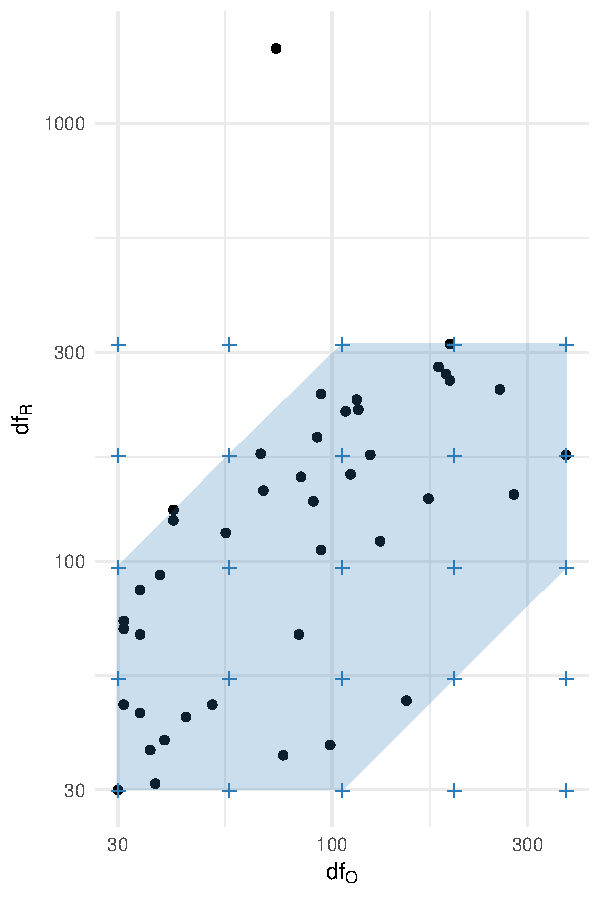
\includegraphics[width=0.5\textwidth]{df}
    \caption{Degrees of freedom in the original and replication experiments where both are at least $30$, on log-scale. The blue region covers all but one study pair, and hence the grid points we choose, marked as ``+'', are generally representative.}
  \label{fig:df}
  \end{figure}

  For each grid point, we simulate a pair of one-sided $t$-tests with the same effect sizes. We generate
  \[
    T_O \sim t_{df_O}(\text{ncp}_O) 1_{\{|T_O| > t_{df_O, \alpha/2}\}} \qquad \text{ and } \qquad T_R \sim t_{df_R}(\text{ncp}_R).
  \]
  Since the original sample size is typically chosen to achieve a certain power, we assume $\text{ncp}_O$ stays small. The type I error rate of the selective $z$-test is given in red in \Cref{fig:t-approx}. The type I error rate can deviate from $0.05$ as the noncentrality parameter grows.
  \begin{figure}[htbp]
    \centering
    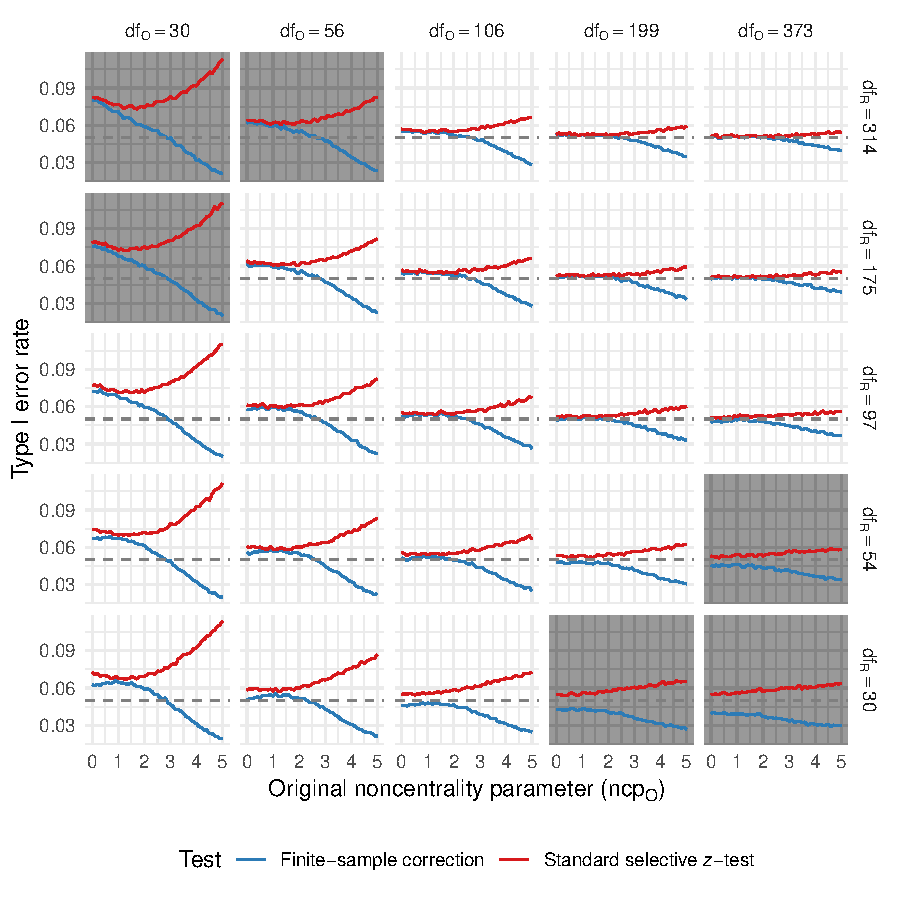
\includegraphics[width=0.8\textwidth]{t-approx}
    \caption{The type I error rate as a function of the noncentrality parameter, based on a simulation. The type I error rate of the simple selective $z$-test is in red, which can deviate from $0.05$ when the noncentrality parameter is large. The type I error rate of the selective $z$-test with our proposed finite sample correction is in blue, and stay mostly controlled. Extreme differences in degrees of freedom, as indicated by the gray background, is absent.}
  \label{fig:t-approx}
  \end{figure}

  This deviation is caused by inaccuracy of approximating a noncentral $t$-distribution with a location-shifted standard Gaussian. We propose a finite sample correction by approximating the distribution of $T_O$ with
  \[
    T_O \sim t_{df_O}(\text{ncp}_O) 1_{\{|T_O| > t_{df_O, \alpha/2}\}} \approx N\left(\text{ncp}_O, 1 + \frac{2\text{ncp}_O^2}{df_O}\right) 1_{\{|T_O| > t_{df_O, \alpha/2}\}}
  \]
  and approximating the distribution of $T_R$ similarly. Note that the distribution of the test statistic relies on the unknown noncentrality parameter, which we replace with a plug-in estimator based on $T_R$: $T_R$ can stand in for $\text{ncp}_R$, as well as $\text{ncp}_O$ through the common effect size. The resulting type I error rate behaves better and is given in blue in \Cref{fig:t-approx}.

  With the finite sample correction, five ($11\%$) studies are rejected. Controlling the false discovery rate at $0.10$, we apply Benjamini--Hochberg  procedure \citeyearpar{Benjamini:1995cd} and rule four ($9\%$) replication studies as inconsistent with the original studies, namely \citet{Dodson:2008ks,vanDijk:2008br,PurdieVaughns:2008en,Farris:2008ev}, generally in line with our results without the finite sample correction. \citet{Farris:2008ev} remains rejected at familywise error rate $0.05$. To check if our assumptions still hold reasonably well, we recreate \Cref{fig:t-approx} with the effective $p$-value threshold of $0.004$ ($=\frac{4}{46} \cdot 0.05$) used in Benjamini--Hochberg procedure and $0.001$ ($=\frac{1}{46} \cdot 0.05$), given in \Cref{fig:t-approx-bh} and \Cref{fig:t-approx-bonf} respectively.
  \begin{figure}[htbp]
    \centering
    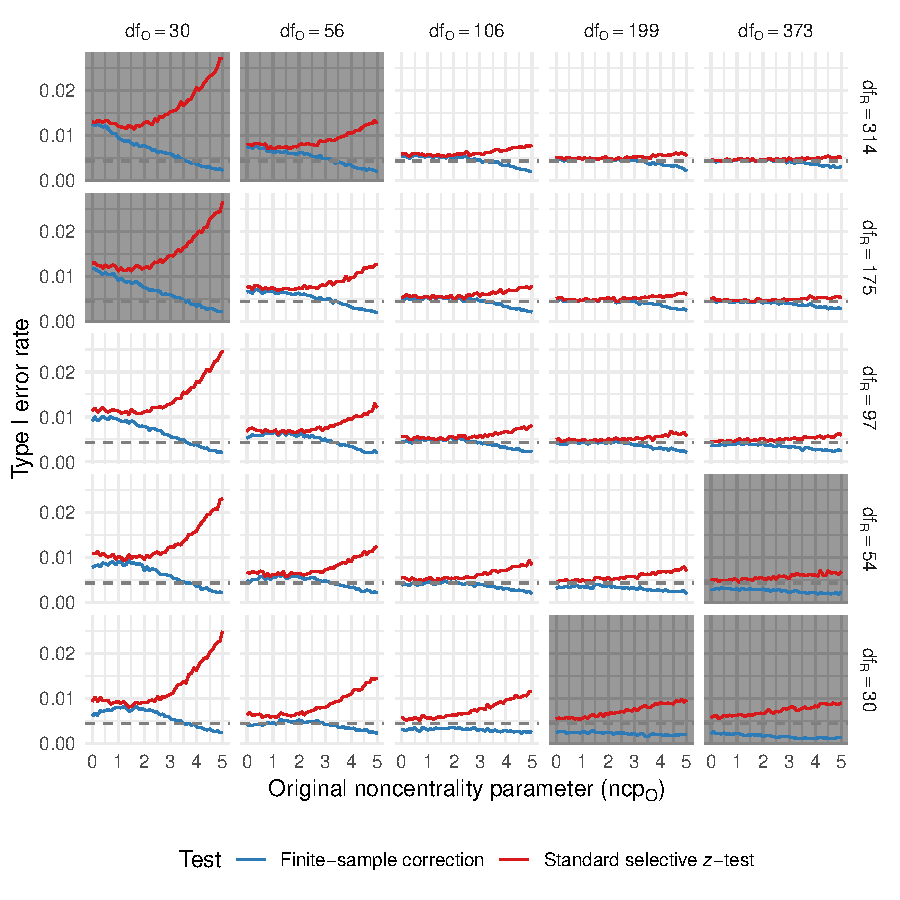
\includegraphics[width=0.8\textwidth]{t-approx-bh}
    \caption{The type I error rate as a function of the noncentrality parameter, based on a simulation. The type I error rate of the simple selective $z$-test is in red, which can deviate from $0.004$ when the noncentrality parameter is large. The type I error rate of the selective $z$-test with our proposed finite sample correction is in blue. Extreme differences in degrees of freedom, as indicated by the gray background, is absent.}
  \label{fig:t-approx-bh}
  \end{figure}
  \begin{figure}[htbp]
    \centering
    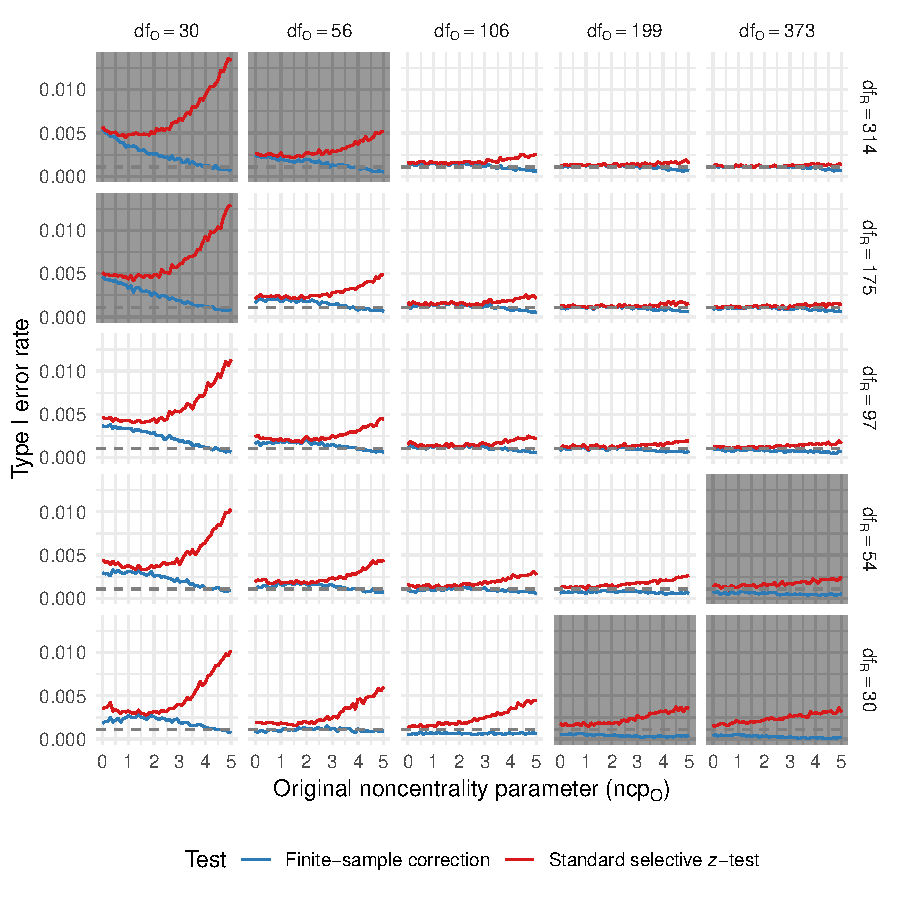
\includegraphics[width=0.8\textwidth]{t-approx-bonf}
    \caption{The type I error rate as a function of the noncentrality parameter, based on a simulation. The type I error rate of the simple selective $z$-test is in red, which can deviate from $0.001$ when the noncentrality parameter is large. The type I error rate of the selective $z$-test with our proposed finite sample correction is in blue. Extreme differences in degrees of freedom, as indicated by the gray background, is absent.}
  \label{fig:t-approx-bonf}
  \end{figure}

  For sake of completeness, we repeat the above plots specifically for the outlier \citep[Study 97;][]{PurdieVaughns:2008en} with exceptionally large replication degree of freedom, in \Cref{fig:t-approx-pv}.
  \begin{figure}[htbp]
    \centering
    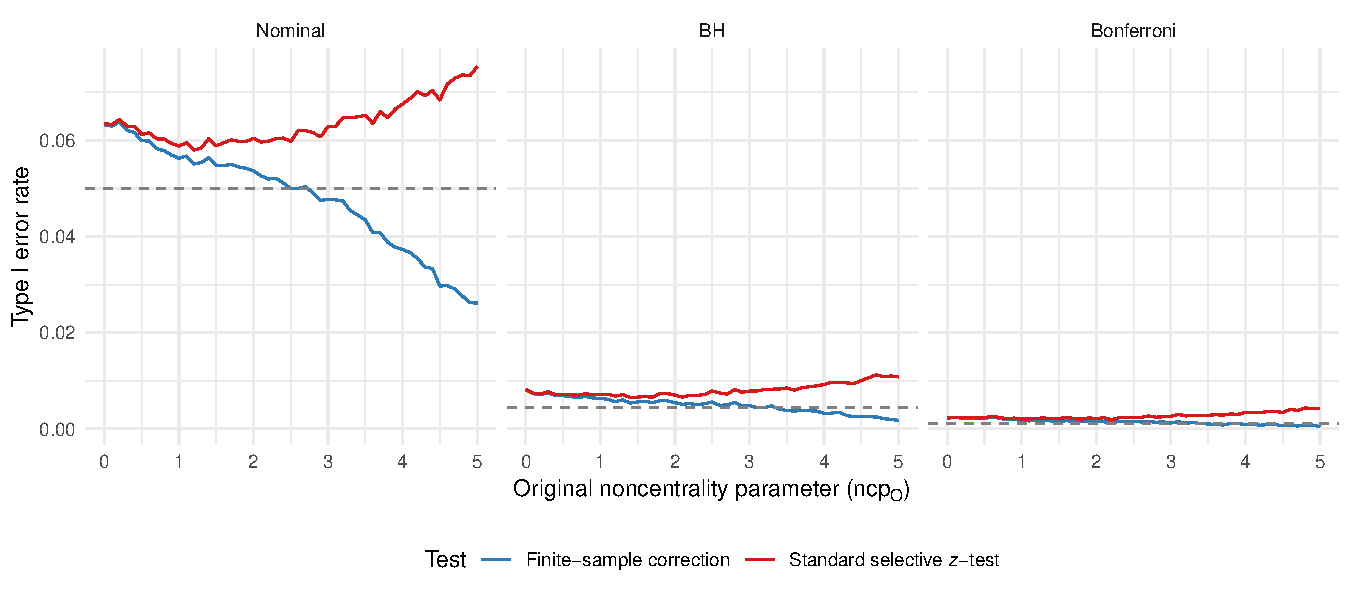
\includegraphics[width=\textwidth]{t-approx-pv}
    \caption{The type I error rate as a function of the noncentrality parameter, based on a simulation. The type I error rate of the simple selective $z$-test is in red and the type I error rate of the selective $z$-test with our proposed finite sample correction is in blue. The error rate is evaluated for a test with the nominal level, the effective level from Benjamini--Hochberg procedure and from Bonferroni correction.}
  \label{fig:t-approx-pv}
  \end{figure}

  Our overestimate, underestimate and confidence interval for the proportion of effect sizes that declined remain the same, but we now estimate conservatively that $14$ ($30\%$) of the effect sizes declined by at least $20\%$ with a $95\%$ lower confidence bound of three ($7\%$).

\Urlmuskip=0mu plus 1mu\relax
\bibliographystyle{plainnat}
\bibliography{papers,additional}

\end{document}
